\subsection{Login}
			\noindent\makebox[\textwidth]{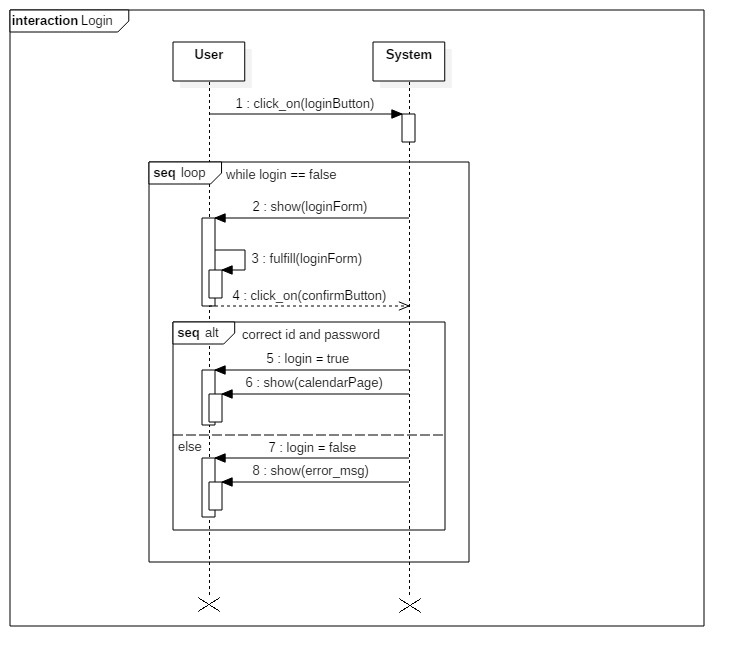
\includegraphics[width=\paperwidth,height=\paperheight,keepaspectratio]{sequence_diagrams/login.png}}
			The login operation is performed only the first time that the application is used. 
			The \textit{system} calculate a unicode that is returned to the client and stored in the \textit{local DB}. In this way the client can be recognized for future operations. 
			The encryption function will be specified below in the document.
\subsection{Authentication functions for each operation}
		\noindent\makebox[\textwidth]{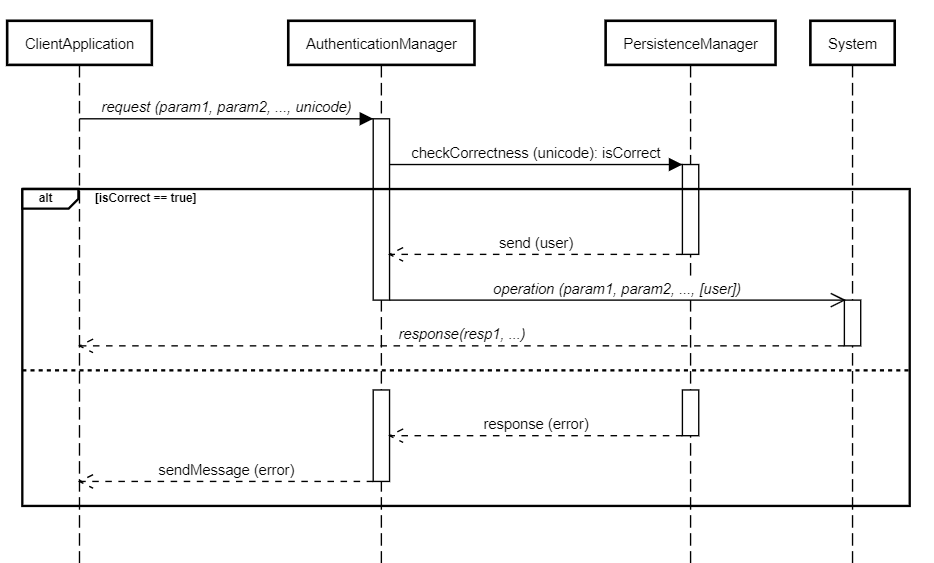
\includegraphics[width=\paperwidth,height=\paperheight,keepaspectratio]{sequence_diagrams/for_each_operation.png}}
		This is a model of how a generic request is taken into account by the system: the \textit{Client} sends the unicode with the other parameters and the \textit{Authentication Manager} performs the check. 
		The \textit{Authentication Manager} forwards the request only if the unicode is correctly recognized.
\subsection{Create event}
		\noindent\makebox[\textwidth]{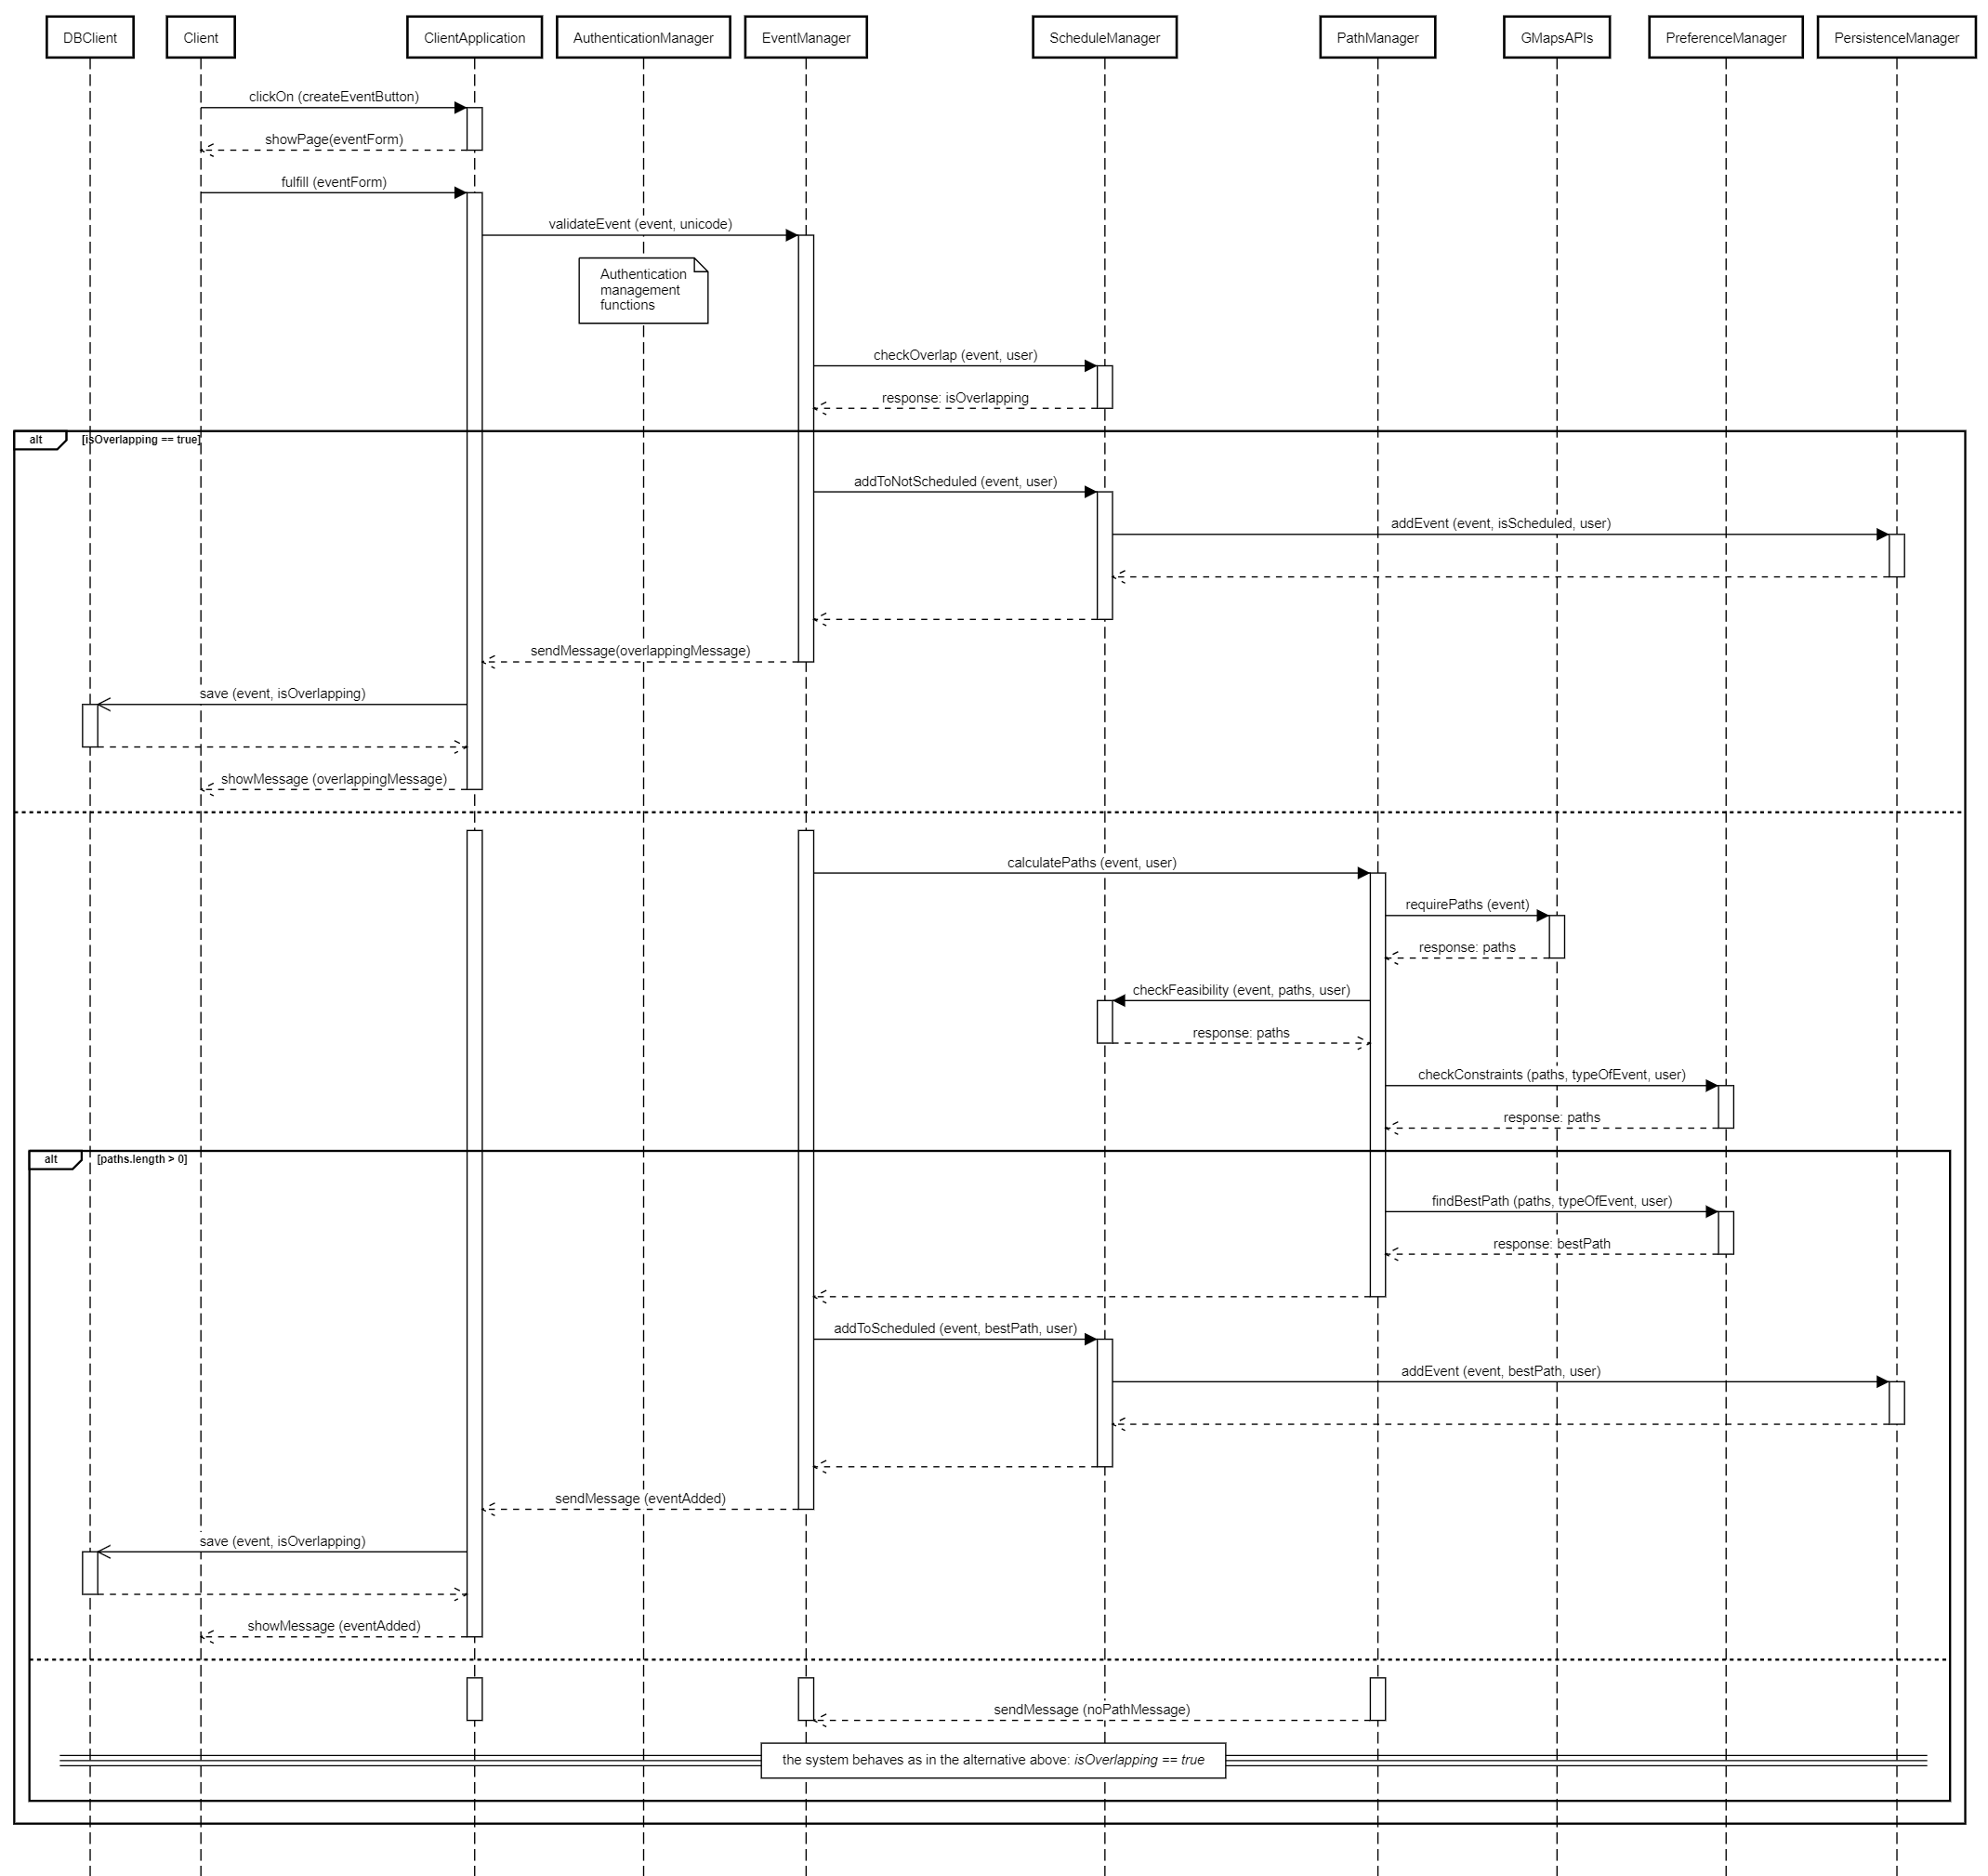
\includegraphics[width=\paperwidth,height=\paperheight,keepaspectratio]{sequence_diagrams/create_event.png}}
\subsection{Arrange trip}
		\noindent\makebox[\textwidth]{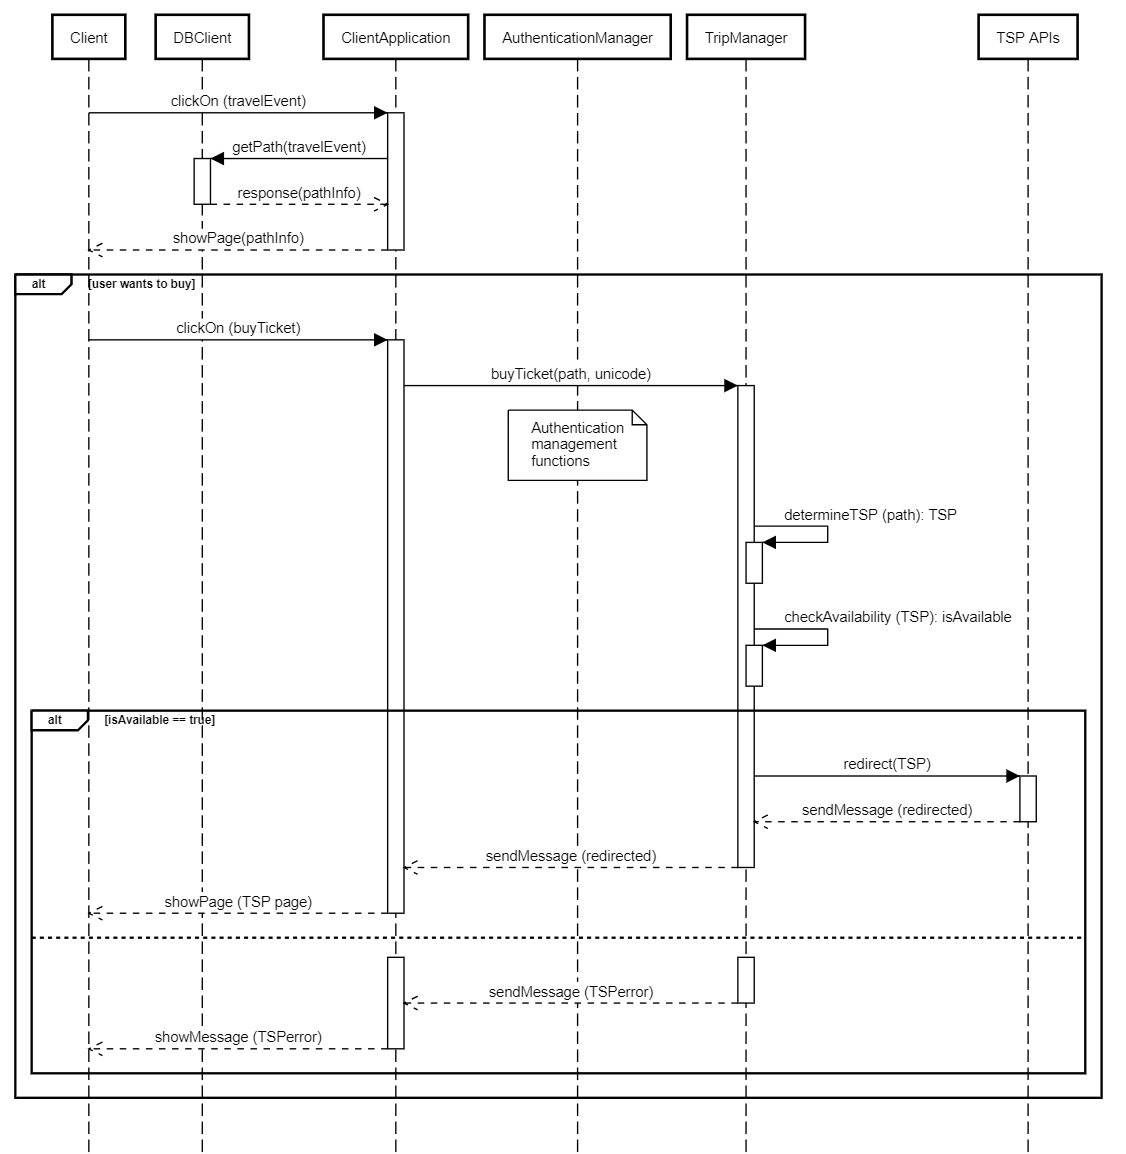
\includegraphics[width=\paperwidth,height=\paperheight,keepaspectratio]{sequence_diagrams/arrange_trip.png}}
\subsection{Obtain feasible paths}
		\noindent\makebox[\textwidth]{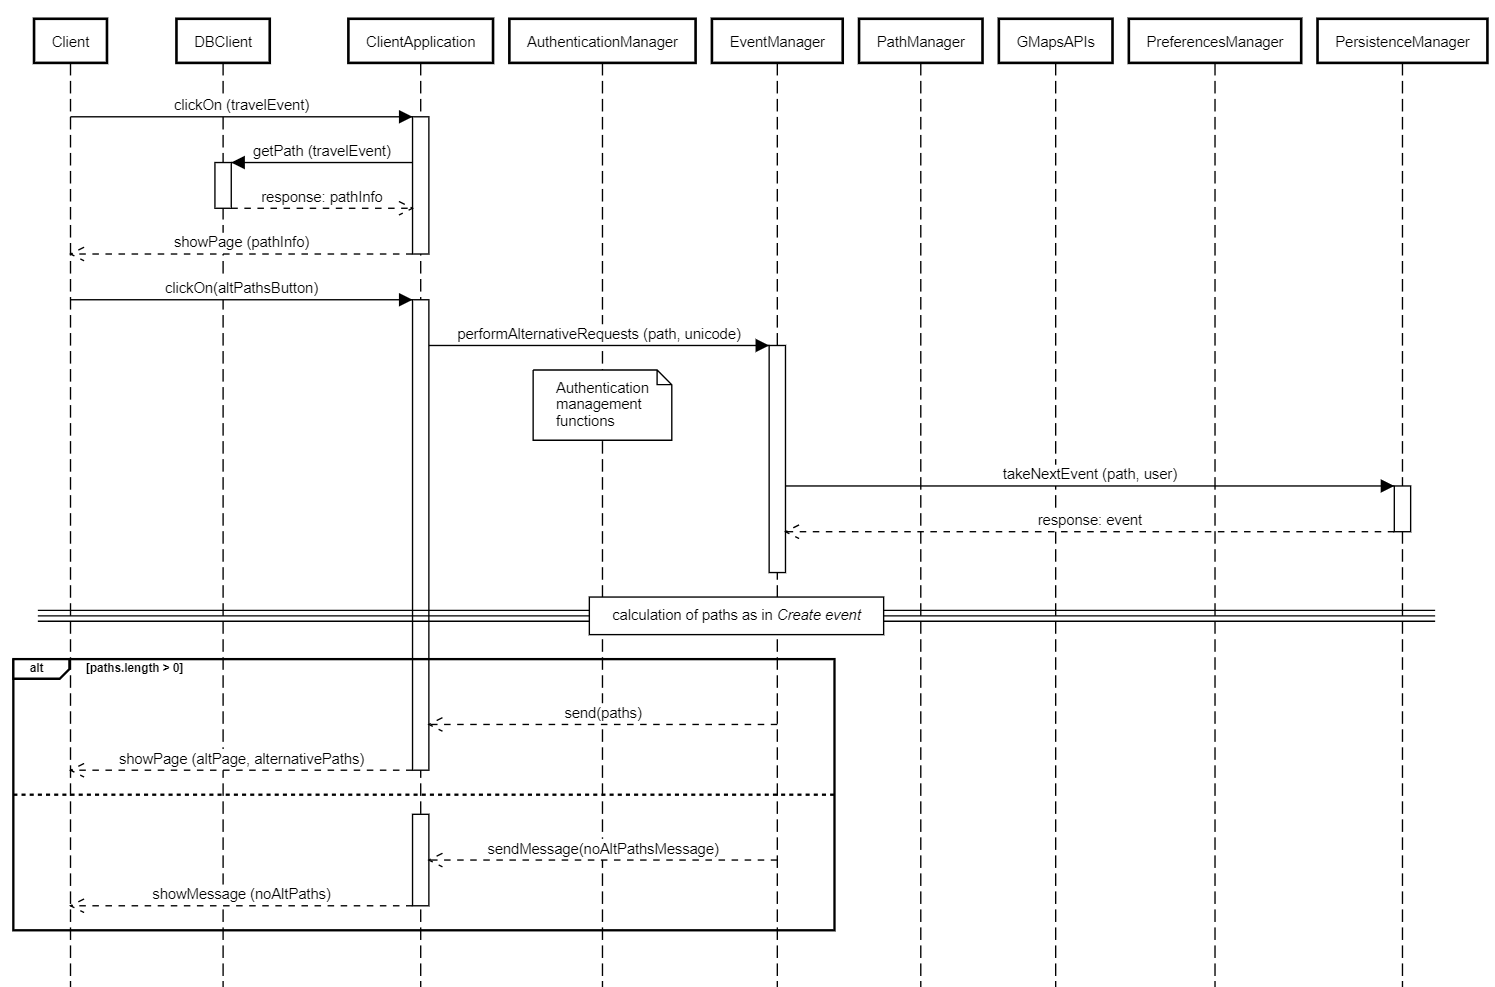
\includegraphics[width=\paperwidth,height=\paperheight,keepaspectratio]{sequence_diagrams/obtain_feasible_paths.png}}
		Because only the best path is stored into \textit{local and server DBs}, if a user wants to see alternative feasible paths, a new calculation of paths is needed. 
		The \textit{system} obtains the event related to the path and then calculates the feasible alternatives with the function of \textit{GMaps} and the checks on feasibility and constraints.
\subsection{Choose between overlapping events}
		\noindent\makebox[\textwidth]{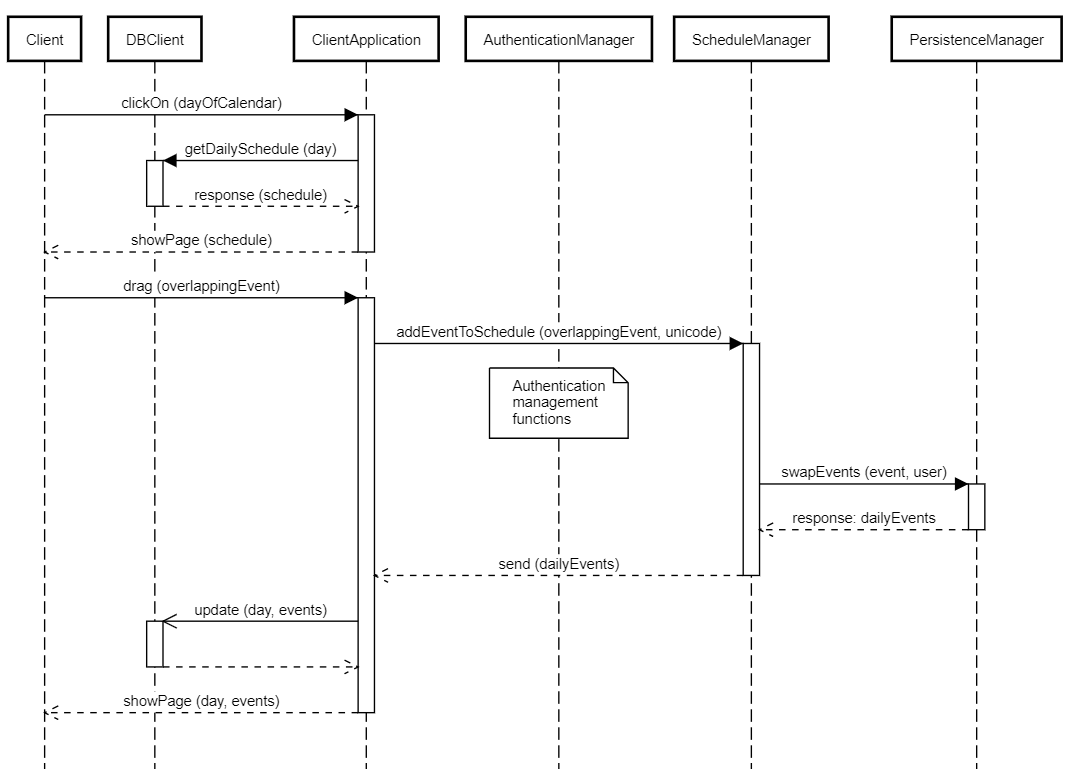
\includegraphics[width=\paperwidth,height=\paperheight,keepaspectratio]{sequence_diagrams/choose_between_overlapping_events.png}}
\subsection{Strike announcement}
		\noindent\makebox[\textwidth]{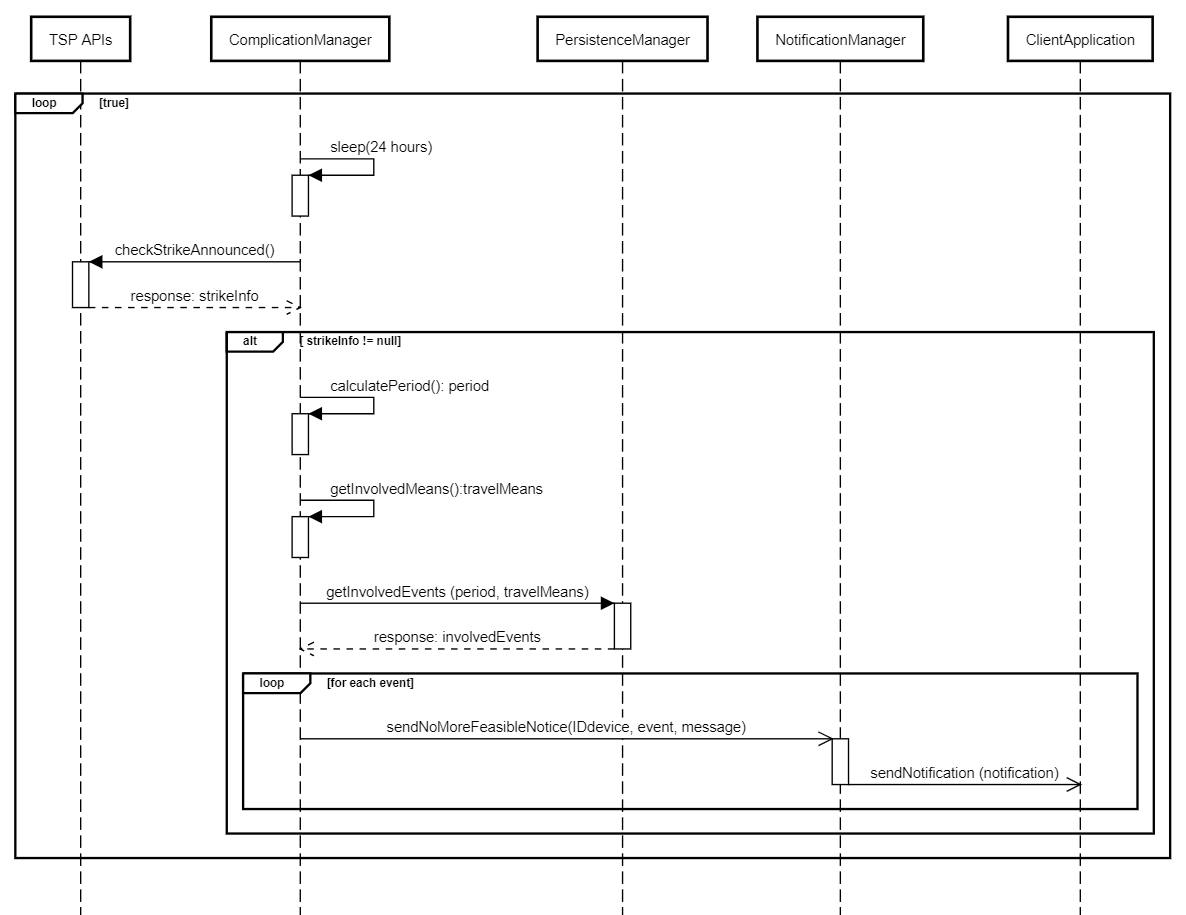
\includegraphics[width=\paperwidth,height=\paperheight,keepaspectratio]{sequence_diagrams/strike_announcement.png}}
		The \textit{Complication Manager} every day performs a list of operations, one of them is to check if a strike for the following days is announced. 
		In case of strike a notification is send for each event stored in the \textit{database} that is involved: to the same user several notifications can be sent. 
		If the user opens the notification, \textit{obtain feasible paths} function, related to the involved event, is called.